\section{Určitý integrál}

Představme si funkci $f(x)$, která má primitivní funkci $F(x)$ (neboli $F'(x)=f(x)$). Reálné číslo \begin{align}
    \boxed{
    \int_a^b f(x) \, \D x = \left[ F(x) \right]_a^b = F(b)-F(a)
    }
\end{align}
se nazývá \textbf{určitý integrál} z funkce $f(x)$ v mezích od $a$ do $b$. 

\textbf{Určitý integrál udává obsah plochy pod křivkou funkce $f(x)$.}
Pokud pracujeme s funkcemi, které nabývají záporných hodnot, musíme dát pozor. \uv{Plocha pod křivkou} bude v takovém případě záporná. Pokud nás tedy zajímá plocha ohraničená nulou a danou funkcí, musíme nejdříve nalézt intervaly, na kterých je funkce kladná (tam se určitý integrál přičítá), a intervaly, na kterých je záporná (tam se odčítá).

\subsection*{Příklady}

\begin{example}[Obsah pravoúhlého trojúhelníka]
    Pomocí určitého integrálu spočítáme obsah pravoúhlého trojúhelníka. Představme si takový objekt jako plochu mezi osami $x$ a $y$ a vhodnou lineární funkcí. Jestliže mají odvěsny délky $a$ a $b$, můžeme třeba zvolit funkci $y(x) = b(1-x/a)$ (ověřte její průsečíky). Obsah pak bude roven \begin{align}
        S = \int_0^a b\left(1-\frac{x}{a}\right) \, \D x = \left[ bx - \frac{bx^2}{2a} \right]_0^a =  ba - \frac{ba^2}{2a} - b \cdot 0 - \frac{b \cdot 0^2}{2a} = ab - \frac{ab}{2} = \frac{ab}{2} \:.
    \end{align}
    Samozřejmě, obsah trojúhelníka je \uv{základna krát výška děleno dvěma}, v případě pravoúhlého trojúhelníka polovina součinu délek odvěsen.
\end{example}

\begin{example}[Obsah obecnějšího trojúhelníka]
    Uvažujme trojúhelník, který vznikne jako plocha ohraničená lineárními funkcemi $y=x$, $y=1-x$ a $y=x/2$. Spočítáme jeho obsah. TODO: obrázek

    Nejdříve najdeme vrcholy trojúhelníku. Zřejmě to jsou body $[0,0]$, $[1/2,1/2]$ a $[2/3,1/3]$.
    Nyní počítáme plochu integrálem \begin{align}
        S = \int_0^{1/2} [x-x/2] \, \D x + \int_{1/2}^{2/3} [1-x - x/2] \, \D x 
        =
        \int_0^{1/2} x/2 \, \D x + \int_{1/2}^{2/3} [1 - 3x/2] \, \D x 
        = \\ =
        [x^2/4]_0^{1/2} + [x-3x^2/2]_{1/2}^{2/3} 
        =
        [\frac{1}{4 \cdot 2^2} - 0 ] + [\frac{2}{3} - 3 \cdot \frac{2^2}{3^2 \cdot 2} - \frac{1}{2} + 3 \cdot \frac{1}{2 \cdot 2^2}] = \frac{1}{48} \:.
    \end{align}
\end{example}


\begin{example}[Obsah kruhu]
    Pomocí určitého integrálu spočítáme obsah kruhu. Kružnice je definovaná jako množina bodů, které mají od středu stejnou vzdálenost. Jestliže umístíme střed do počátku souřadnic, je vzdálenost bodu $(x,y)$ dána Pythagorovou větou $x^2 + y^2$, tato vzdálenost je stále konstantní a je rovna $R^2$. Proto rovnice kružnice bude $x^2 + y^2 = R^2$. Položme pro jednoduchost $R=1$.
    Z tohoto vztahu můžeme zkusit vyjádřit křivku jako funkci $y(x)$. Zřejmě máme dvě možnosti: $y = \pm \sqrt{1-x^2}$. Zamyslíme-li se nad obrázkem, bude nám stačit uvažovat čtvrtkruh - spočítáme obsah pod křivkou $y = \sqrt{1-x^2}$ v intervalu $[0,1]$ a výsledek vynásobíme čtyřmi.

    Je tedy třeba spočítat \begin{align}
        I = \int_0^1 \sqrt{1-x^2} \, \D x \:.
    \end{align}
    Můžeme postupovat například metodou per-partes s využitím jedničky: $u=\sqrt{1-x^2}$, $u'=\frac{-x}{\sqrt{1-x^2}}$, $v'=1$, $v=x$. Tedy \begin{align}
        \int_0^1 \sqrt{1-x^2} \, \D x = \left[ x \sqrt{1-x^2}\right]_0^1 - \int_0^1 \frac{-x}{\sqrt{1-x^2}} \cdot x \, \D x = 0 + \int_0^1 \frac{x^2}{\sqrt{1-x^2}} \, \D x \:.
    \end{align}
    Nyní využijeme šikovného rozpisu $x^2 = x^2-1+1 = -(1-x^2) + 1$. Dostaneme \begin{align}
        \int_0^1 \frac{x^2}{\sqrt{1-x^2}} \, \D x = -\int_0^1 \frac{1-x^2}{\sqrt{1-x^2}} \, \D x + \int_0^1 \frac{1}{\sqrt{1-x^2}} \, \D x 
        = \\ = 
         -\int_0^1 \sqrt{1-x^2} + \left[ \arcsin x \right]_0^1 = - I + \left[ \arcsin 1 - \arcsin 0 \right] = - I + \frac{\pi}{2} \:.
    \end{align}
    Dostali jsme rovnici $I = - I + \frac{\pi}{2}$. Odtud \begin{align}
        I = \frac{\pi}{4} \:.
    \end{align}
    To je obsah jedné čtvrtiny kruhu. Celý kruh má proto obsah $S = \pi$.
\end{example}

\subsection*{Aplikace}

\begin{example}[Přebytek spotřebitele]
    Uvažujme křivku poptávky $D(Q)$ a úrovní ceny $P^\star$, které se protínají v bodě $Q^\star$. Přebytek spotřebitele (total consumer surplus) $\mathsf{TCS}$ udává rozdíl mezi tím, kolik by byl ochoten kupující zaplatit, a kolik zaplatí ve skutečnosti. V grafu ho představuje plocha pod poptávkovou křivkou a nad úrovní ceny, neboli \begin{align}
        \mathsf{TCS} = \int_0^{Q^\star} [D(Q) - P^\star] \, \D Q = \int_0^{Q^\star} D(Q) \, \D Q  - P^\star Q^\star \:.
    \end{align}
\end{example}

\begin{figure}[H]
    \centering
    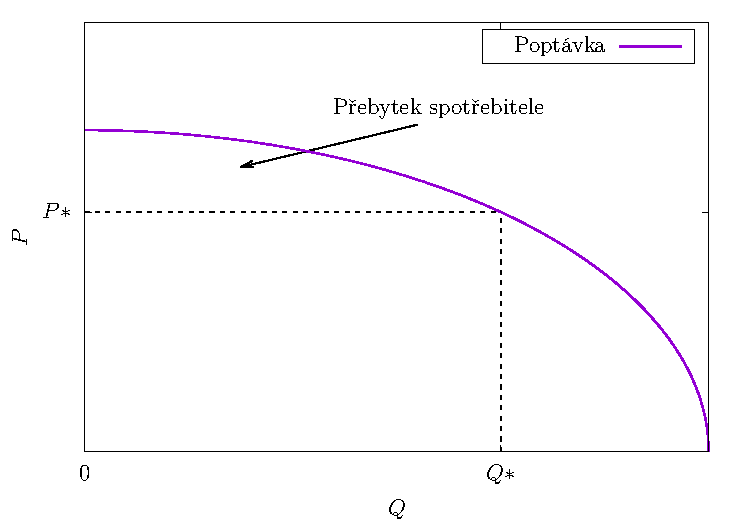
\includegraphics[scale = 0.8]{Gnuplot/Figures/prebytek-spotrebitele-graf.pdf}
    \caption{Přebytek spotřebitele je dán plochou mezi křivkou poptávky a danou úrovní ceny $P^\star$.}
\end{figure}

\begin{example}[Ztráta mrtvé váhy]
    Uvažujme křivku nabídky $S(Q)$ a poptávky $D(Q)$, které se protínají v bodě $Q_E$. Pokud vláda uvalí na daný statek daň, sníží se prodávané množství na $Q_T$. Výsledkem tohoto snížení je, že část potenciálního prospěchu z obchodu mezi kupujícím a prodávajícím se nerealizuje. Tento ztracený prospěch z obchodu tvoří ztrátu mrtvé váhy (deadweight loss) $\mathsf{DL}$. V grafu nabídky a poptávky se jedná o plochu mezi funkcemi $D(Q)$ a $S(Q)$ ohraničenou body $Q_T$ a $Q_E$, neboli \begin{align}
        \mathsf{DL} = \int_{Q_T}^{Q_E} \left[ D(Q) - S(Q) \right] \, \D Q \:.
    \end{align}
\end{example}

% TODO: obrázek přebytku spotřebitele

% TODO: dodělat plochu pod křivkami v obrázku
\begin{figure}[H]
    \centering
    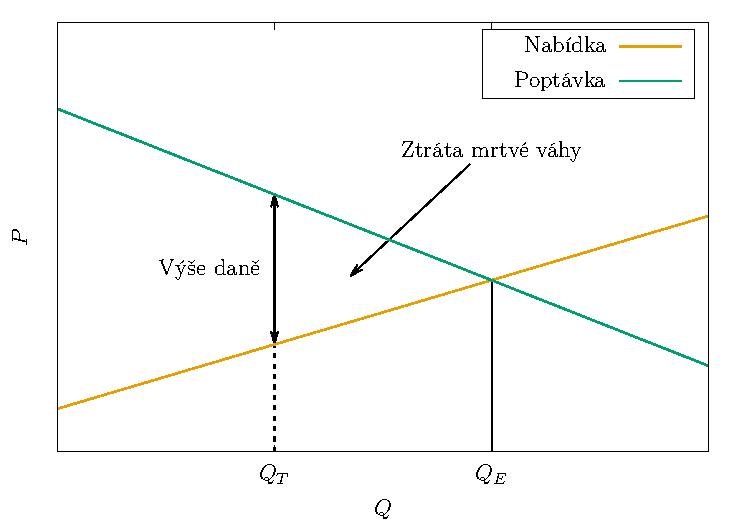
\includegraphics[scale = 0.8]{Gnuplot/Figures/ztrata-mrtve-vahy-graf.pdf}
    \caption{Ztráta mrtvé váhy je dána plochou mezi křivkami nabídky a poptávky mezi rovnovážnou cenou a cenou po zdanění.}
\end{figure}

\section*{Nevlastní integrál}

Někdy se setkáváme se situacemi, kde lze spočítat plochu grafu funkce i na neomezeném intervalu (\uv{od nějakého čísla do nekonečna}). Nebo se lze setkat s funkcemi, které jsou neomezené na okolí nějakého bodu, a přesto lze definovat obsah pod grafem. V takovém případě mluvíme o \textbf{nevlastních integrálech}. Strategie je jednoduchá: zvolíme si konečné číslo jako mez tak, aby v integrálu nebyl žádný problém, potom integrál vypočítáme na tomto intervalu a nakonec zkusíme provést limitní přechod.

\begin{example}
    Spočítejme integrál
    \begin{align}
        \int_1^\infty \frac{1}{x^5} \, \D x \:.
    \end{align}
    Zvolíme si (velké) číslo $a$, spočítáme integrál v mezích $[1,a]$ a nakonec pošleme $a$ do nekonečna.
    \begin{align}
        \int_1^a \frac{1}{x^5} \, \D x = \left[ -\frac{1}{4x^4} \right]_1^a
        = \left[ - \frac{1}{4a^4} + \frac{1}{4} \right] = \frac{1}{4} -\frac{1}{4a^4}
    \end{align}
    a po limitním přechodu \begin{align}
        \int_1^\infty \frac{1}{x^5} \, \D x = \lim_{a \rightarrow \infty} \left[ \frac{1}{4} -\frac{1}{4a^4} \right] = \frac{1}{4} - 0 = \frac{1}{4} \:.
    \end{align}
\end{example}

\begin{example}
    Spočítejme integrál \begin{align}
        \int_0^1 \frac{1}{\sqrt{x}} \, \D x \:.
    \end{align}
    Problém máme v nule, protože nulou nemůžeme dělit a funkce v tomto bodě není definovaná. Opět si zvolíme (malé) číslo $b$, spočítáme integrál v mezích $[b,1]$ a pak pošleme $b$ k nule.
    \begin{align}
        \int_b^1 \frac{1}{\sqrt{x}} \, \D x = \left[ 2 \sqrt{x} \right]_b^1 = 2 - 2 \sqrt{b} \:,
    \end{align}
    takže \begin{align}
        \int_0^1 \frac{1}{\sqrt{x}} \, \D x = \lim_{b \rightarrow 0+} 2 - 2 \sqrt{b} = 2 \:.
    \end{align}
\end{example}

\begin{example}
    Pokusme se spočítat \begin{align}
        \int_1^\infty \frac{1}{x} \, \D x \:.
    \end{align}
    Opět zvolíme (velké) číslo $a$, \begin{align}
        \int_1^a \frac{1}{x} \, \D x = \left[ \log x \right]_1^a = \log a - \log 1 = \log a \:.  
    \end{align}
    Pokud provedeme limitní přechod, dostaneme \begin{align}
        \int_1^\infty \frac{1}{x} \, \D x = + \infty \:.
    \end{align}
    V tomto případě říkáme, že \textbf{integrál diverguje}.
\end{example}

\begin{example}
    Pokusme se spočítat \begin{align}
        \int_0^\infty \cos x \, \D x \:.
    \end{align}
    Obvyklým postupem spočteme \begin{align}
        \int_0^a \cos x \, \D x = \left[ \sin x \right]_0^a = \sin a \:.
    \end{align}
    Vidíme, že limitní přechod $a \rightarrow \infty$ nemůžeme provést. Je to dáno tím, že funkce $\sin x$ \textbf{osciluje}. Nemůžeme určit plochu pod grafem až do nekonečna, protože se zvětšujícím se $a$ se plocha nejprve zvětšuje, pak zase zmenšuje, pak zase zvětšuje, \dots
\end{example}

\subsection*{Poznámky}

\begin{itemize}
    \item V tomto kurzu mluvíme o neurčitém integrálu (primitivní funkci) a určitém integrálu (čísle, které vyjadřuje plochu pod grafem). Ve skutečnosti se dá pojem obsahu (objemu) zavést různými způsoby. Matematikové rozlišují tři hlavní typy integrálů: Newtonův, Riemannův a Lebesgueův. Každý z nich se vyznačuje drobnými zvláštnostmi (např. Newtonův si neumí poradit s velkým počtem nespojitostí, Riemannův si neporadí s neomezenými intervaly a Lebesgueův si neporadí s oscilujícími funkcemi). Jedná se však spíše o teoretickou záležitost. V praxi se integrály počítají všechny stejným způsobem.
    \item Počítačové algoritmy umějí integrovat numericky (tzv. kvadratura). Nejjednodušší metoda je rozdělit si interval na dostatečně malé obdélníčky a sčítat jejich obsahy.
    \item Integrál se dá zobecnit do více dimenzí. Pro funkce dvou proměnných se dá definovat \textbf{dvojný integrál} $\iint_M f(x,y)\, \D x \D y$, který reprezentuje objem ohraničený funkcí $f(x,y)$ na nějaké množině $M$ (obdélník, kruh, složitější obrazec). Je to naprosto zásadní technika pro výpočet všemožných obsahů, povrchů, objemů, těžiště, setrvačných vlastností a celkově je potřeba všude, kde se bere v potaz nějaká úhrnná veličina.
    \item Na obdélníku $O = [a,b] \times [c,d]$ se dá počítat dvojný integrál z $f(x,y)$ jednoduše - nejprve se integruje podle jedné proměnné a poté podle druhé proměnné (dokonce nezáleží na pořadí):
    \begin{align}
        \iint_{O} f(x,y) \, \D x \D y = \int_a^b \left[ \int_c^d f(x,y) \, \D y \right] \, \D x = \int_c^d \left[ \int_a^b f(x,y) \, \D x \right] \, \D y \:.
    \end{align}
    \item Matematická oblast zabývající se integrálem se nazývá \textbf{teorie míry}. Jde ruku v ruce s \textbf{teorií pravděpodobnosti a statistiky}. Myšlenka je založená na tom, že pravděpodobnost má stejné vlastnosti jako objem. Jakýkoli problém z pravděpodobnosti lze tedy geometrizovat - převést na problém výpočtu nějakého \uv{zobecněného objemu}. Koho zajímá pravděpodobnost, musí umět dobře rozumět integrálům!
\end{itemize}

